\ifx\allfiles\undefined
\documentclass{article}
\usepackage{graphicx}
\usepackage{geometry}
\usepackage{hyperref}
\usepackage{amssymb}
\usepackage{booktabs}
\usepackage{tabularx}
\usepackage{amsthm}
\usepackage{amsmath}
\usepackage{enumitem}
\usepackage{tikz}
\usetikzlibrary{automata, positioning, arrows}

\geometry{left=1.2in, right=1.2in, top=1.5in, bottom=1.5in}
\linespread{1.5}%行距

% 设置列表环境的上下间距
\setenumerate[1]{itemsep=5pt,partopsep=0pt,parsep=\parskip,topsep=5pt}
\setitemize[1]{itemsep=5pt,partopsep=0pt,parsep=\parskip,topsep=5pt}
\setdescription{itemsep=5pt,partopsep=0pt,parsep=\parskip,topsep=5pt}

\theoremstyle{definition}
\newtheorem{defn}{\textbf{\textit{def}}}[section]
\newtheorem{prop}{\textbf{\textit{prop}}}[section]
\newtheorem{thm}[defn]{\textbf{\textit{thm}}}

\newtheorem{lemma}{lemma}[section]% 引理 推论 准则 共用一个编号计数
\newtheorem{corollary}[lemma]{\textbf{\textit{corollary}}}
\newtheorem{criterion}[lemma]{\textbf{\textit{criterion}}}

\newtheorem{proposition}{\textbf{\textit{proposition}}}[section]
\newtheorem{example}{\textbf{\textit{e.g.}}}[section]
\newtheorem{exercises}{\textbf{\textit{exercises}}}[section]
\newtheorem*{remark}{\textbf{\textit{remark}}}

\newenvironment{solution}{\par{\textit{solution}}\;}{\qed\par}

\def\R{\mathbb{R}} % 实数域
\def\N{\mathbb{N}} % 自然数域
\def\Q{\mathbb{Q}} % 有理数域
\def\eps{\varepsilon} %ε

\graphicspath{ {pictures/},{../pictures/}}  % 配置图形文件检索目录
\begin{document}
\setcounter{section}{1}
\else
\fi
\section{Automata and Language}
\subsection{Finite Automaton}
\begin{example}
    \textit{Automatic Door\\}
    \bgpic    
    \node[state] (q0) {$closed$}; 
        \node[state] (q1) [right=of q0] {$open$};
        \path[->]
            (q0) edge[loop left] node {$neither$} ()
            (q1) edge[loop right] node {$front,rear,both$} ()
            (q0) edge[bend left] node {$front,rear,both$} (q1) % 从 q0 到 q1 的转换
            (q1) edge[bend left] node {$neither$} (q0); % 从 q1 到 q0 的转换
    \end{tikzpicture}

    \bgtbl
            \toprule
        $~$ & $front$ & $rear$ & $both$ & $neither$ \\
        \midrule
        $front$ & $\checkmark$ & $\times$ & $\checkmark$ & $\times$\\
        $rear$ & $\times$ & $\checkmark$ & $\checkmark$ & $\times$\\
            \bottomrule
        \end{tabularx}
        \label{tab:mytable}
    \end{table}
\end{example}

\begin{example}
    \textit{L = $\{w\in \{0,1\}^*|w = w_1w_2\cdots w_n,w_n = 0\}$\\}
    \bgpic  
        \node[state,accepting] (A)                    {$q_0$};
        \node[state]         (B) [right of=A]       {$q_1$};
      
        \path (A) edge [bend left]  node {1} (B)
                  edge [loop above] node {0} (A)
              (B) edge [bend left]  node {0} (A)
                  edge [loop below] node {1} (B);
    \end{tikzpicture}

    \begin{remark}
        \textit{$q_0:$ accepted state}
    \end{remark}

    \textit{$Q = \{q_0,q_1\},\Sigma = \{0,1\},\delta: Q\times \Sigma \rightarrow Q$}
    \bgtbl
            \toprule
        $~$ & $0$ & $1$  \\
        \midrule
        $q_0$ & $q_0$ & $q_1$ \\
        $q_1$ & $q_0$ & $q_1$ \\
            \bottomrule
        \end{tabularx}
    \end{table}
\end{example}


\begin{defn}
    \textit{(finite automaton)}

    \textit{A \textbf{finite automaton} is a 5-tuple ($Q,\Sigma,\delta,q_0,F$), where:}

    \begin{enumerate}
        \item \textit{Q is a finite set called the states}
        \item \textit{$\Sigma$ is the alphabet}
        \item \textit{$\delta:Q\times \Sigma \rightarrow Q$ is the transition function}
        \item \textit{$q_0$ is the start state }
        \item \textit{$F\subseteq Q$ is the set of accept states}
    \end{enumerate}
\end{defn}

\begin{defn}
    \textit{Let $M = (Q,\Sigma,\delta,q_0,F)$ be a finite automaton, let w = $w_1w_2\cdots w_n$ be a string, where each $w_i \in \Sigma$.}

    \textit{Then M accept w if there is a sequence of states $r_0,r_1,\cdots,r_n\in Q,$ such that:}

    \begin{enumerate}
        \item $r_0=q_0$
        \item \textit{$\delta(r_i,w_{i+1}) = r_{i+1}$, for $i = 0,1,2,\cdots,n-1$}
        \item $r_n \in F$
    \end{enumerate}
\end{defn}

\begin{defn}
    \textit{If L is the set of strings that M accepts, we say L is the language of M, and write L(M) = L, we say M recognizes/decides/accepts L.}

    \textit{If M accepts no string, it recognizes one language namely, the empty language.}
\end{defn}

\begin{example}
    \textit{L = $\{w\in \{0,1\}^*|w = w_1w_2\cdots w_n,w_n = w_1\}$\\}
    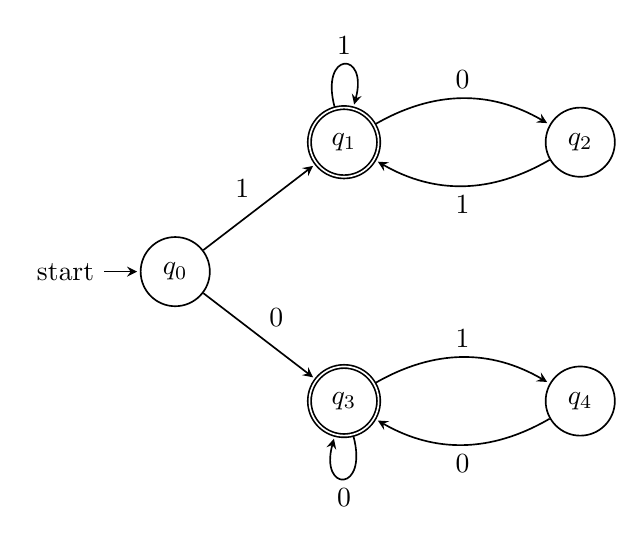
\begin{tikzpicture}[->,>=stealth,shorten >=1pt,auto,node distance=3cm,semithick]
        \tikzstyle{every state}=[fill=white,draw=black,text=black]
      
        \node[state,initial] (A)                    {$q_0$};
        \node[state,accepting]         (B) [above right = 1cm and 1.5cm of A]       {$q_1$};
        \node[state,accepting]         (C) [below right = 1cm and 1.5cm of A] {$q_3$};
        \node[state]         (D) [right of=B]       {$q_2$};
        \node[state]         (E) [right of=C]       {$q_4$};

        \path (A) edge  node {1} (B)
                  edge  node {0} (C)
              (B) edge [loop above] node {1} (B)
                  edge [bend left]  node {0} (D)
              (C) edge [bend left]  node {1} (E)
                  edge [loop below] node {0} (C)
              (D) edge [bend left]  node {1} (B)
              (E) edge [bend left]  node {0} (C);
      \end{tikzpicture}
\end{example}

\subsection{Regular Language}
\begin{defn}
    \textit{(regular language) $L \subseteq \Sigma^*$ is a \textbf{regular language} if there is a finite automaton that accepts L}

    \textit{Let $A,B\subseteq\Sigma^*$, define:}

    \begin{itemize}
        \item \textit{(union) $A\cup B = \{x\in \Sigma^*|x\in A$ or $x\in B\}$}
        \item \textit{(concatenation) AB = $\{xy|x\in A,y\in B\}$}
        \item \textit{(star) $A^* = \{x_1x_2\cdots x_k| k\geq 0,x_1,x_2,\cdots,x_k\in A\}$}
    \end{itemize}
\end{defn}

\begin{thm}
    \textit{If $A_1,A_2$ are regular languages, so is $A_1\cup A_2$}

    \begin{proof}
        \textit{Let $M_1 = (Q_1,\Sigma_1,\delta_1,q_{10},F_1)$ accepts $A_1$, $M_2 = (Q_2,\Sigma_2,\delta_2,q_{20},F_2)$ accepts $A_2$, construct M = $(Q,\Sigma,\delta,q_0,F)$:}
        \begin{enumerate}
            \item $Q = Q_1\times Q_2 = \{(r_1,r_2)|r_1\in Q_1,r_2\in Q_2\}$
            \item \textit{$\delta:Q\times \Sigma \rightarrow Q$ is defined as for each $(r_1,r_2)\in Q$, and each $a \in \Sigma$, let $\delta ((r_1,r_2),a) = (\delta_1(r_1,a),\delta_2(r_2,a))$}
            \item $q_0 = (q_{10},q_{20})$
            \item \textit{$F = \{(r_1,r_2)|r_1\in F_1$ or $r_2\in F_2\}$}
        \end{enumerate}
    \end{proof}
    \begin{remark}
        \textit{so is $A\cap B = \overline{\overline{A}\cup\overline{B}}$\footnote{\textit{proof of the closure under complement will be mentioned later}}}
    \end{remark}
\end{thm}

\subsection{DFA and NFA}

\begin{thm}
    \textit{If $A_1,A_2$ are regular languages, so is $A_1A_2$}

    \begin{itemize}
        \item \textit{\textbf{DFA}: deterministic finite automaton}
        \item \textit{\textbf{NFA}: nondeterministic\dots}
    \end{itemize}
    
    \textcolor{red}{\textbf{\textit{If at least one of these processes accepts, then the entire computation accepts.}}}
    \begin{example}
        \textit{NFA:\\}
        \bgpic
            \node[state,initial] (A)                    {$q_1$};
            \node[state]         (B) [below right of=A]       {$q_2$};
            \node[state]         (C) [above right of=B]       {$q_3$};
            \node[state,accepting]         (D) [below right of=C] {$q_4$};

          
            \path (A) edge              node {1} (B)
                      edge [loop above] node {$0,1$} (A)
                  (B) edge              node {$0,\eps$} (C)
                  (C) edge              node {1} (D)
                  (D) edge [loop right] node {$0,1$} (D);
        \end{tikzpicture}

        \textit{input: $010110$\\}
        \begin{figure}[htbp]
            \centering \includegraphics[scale = 0.3]{2.1.png}
            \caption{\textit{The computation of NFA on input 010110}}
        \end{figure}

        \begin{figure}
            \centering \includegraphics[scale = 0.8]{2.2.png}
            \caption{\textit{Deterministic and nondeterministic computations with an accepting branch}}
        \end{figure}
          
    \end{example}
\end{thm}

\begin{remark}
    \textit{If a language can be accepted by DFA, then its time complexity is O(n), space complexity is O(1).}
\end{remark}

\begin{example}
    \textit{Let A be the language consisting of all strings over $\{0,1\}$ containing a $1$ in the third position from the end (e.g., $000100$ is in A but $0011$ is not). The following four-state NFA recognizes A.}
    
    \bgpic
        \node[state,initial] (A)                    {$q_0$};
        \node[state]         (B) [right of=A]       {$q_1$};
        \node[state]         (C) [right of=B]       {$q_2$};
        \node[state,accepting]         (D) [right of=C]       {$q_3$};
    
        \path (A) edge              node {1} (B)
                edge [loop above]   node {$0,1$} (A)
              (B) edge              node {$0,1$} (C)
              (C) edge              node {$0,1$} (D);
    \end{tikzpicture}
\end{example}

\begin{example}
    \textit{$L = \{0^k,2|k~or~3|k\}$\\}
    \bgpic
        \node[state,initial] (A)                    {$q_0$};
        \node[state,accepting]         (B) [above right = 0.5cm and 1.5cm of A]       {$q_1$};
        \node[state]         (C) [right of=B]       {$q_2$};
        \node[state,accepting]         (D) [below right = 0.5cm and 1.5cm of A]       {$q_3$};
        \node[state]         (E) [right of=D]       {$q_4$};
        \node[state]         (F) [below right = 1cm and 0.68cm of D]       {$q_5$};
      
        \path (A) edge [bend left]  node {$\eps$} (B)
                  edge [bend left]  node {$\eps$} (D)
              (B) edge [bend left]  node {0} (C)
              (C) edge [bend left]  node {0} (B)
              (D) edge [bend left]  node {0} (E)
              (E) edge [bend left]  node {0} (F)
              (F) edge [bend left]  node {0} (D);
      \end{tikzpicture}
\end{example}

\begin{defn}
    \textit{(NFA)}

    \textit{An \textbf{NFA} is a 5-tuple $(Q,\Sigma,\delta,q_0,F)$,where:}

    \begin{enumerate}
        \item \textit{Q is a finite set of states}
        \item \textit{$\Sigma$ is the alphabet}
        \item \textit{$\delta: Q\times(\Sigma\cup\{\eps\})\rightarrow P(Q)$ is the transive function}
        \item \textit{$q_0 \in Q$ is the start state}
        \item \textit{$F \subseteq Q$ is the set of accept states}
    \end{enumerate}
\end{defn}

\begin{remark}
    \textit{$P(Q)$ is the collection of all the subsets of Q (power set)}
\end{remark}

\begin{itemize}
    \item \textit{variant1: $\delta: Q\times\Sigma^*\rightarrow Q$\\We guarantee there is at most one applicable transition.}
    \item \textit{variant2: If there are multiple applicable transitions,non-deterministically choose one.}
\end{itemize}

\begin{defn}
    \

    \textit{Let $N = (Q,\Sigma,\delta,q_0,F)$ be an NFA, and let $w\in \Sigma ^*$. Say N accepts w if we can write $w = y_1y_2\cdots y_m$, where $y_i\in \Sigma\cup\{\eps\}$, and there exist $r_0,r_1,\cdots,r_m\in Q$, such that:}

    \begin{enumerate}
        \item $r_0 = q_0$
        \item \textit{$r_{i+1} \in \delta(r_i,y_{i+1})$ for $i = 0,1,\cdots,m-1$}
        \item $r_m\in F$
    \end{enumerate}
\end{defn}

\begin{example}
    \textit{$Q = \{q_0,q_1,q_2,q_3\},\Sigma = \{0,1\},F = \{q_3\},\delta:Q\times\Sigma\rightarrow Q$\\}
    \bgpic
        \node[state,initial] (A)                    {$q_0$};
        \node[state]         (B) [right of=A]       {$q_1$};
        \node[state]         (C) [right of=B]       {$q_2$};
        \node[state,accepting]         (D) [right of=C]       {$q_3$};
    
        \path (A) edge              node {1} (B)
                edge [loop above]   node {$0,1$} (A)
              (B) edge              node {$0,\eps$} (C)
              (C) edge              node {$1$} (D)
              (D) edge[loop above]  node {$0,1$} (D);
    \end{tikzpicture}

    \bgtbl
            \toprule
        $q$\textbackslash$\Sigma$ & $0$ & $1$ &$\eps$  \\
        \midrule
        $q_0$ & $\{q_0\}$ & $\{q_0,q_1\}$ & $\emptyset$\\
        $q_1$ & $\{q_2\}$ & $\emptyset$ & $\{q_2\}$\\
        $q_2$ & $\emptyset$ & $\{q_3\}$ & $\emptyset$\\
        $q_3$ & $\{q_3\}$ & $\{q_3\}$ & $\emptyset$\\
            \bottomrule
        \end{tabularx}
    \end{table}
\end{example}

\begin{thm}
    \textit{Every NFA has an equivalent DFA}

    \begin{proof}
          \textit{Let $N = (Q,\Sigma,\delta,q_0,F)$ be the NFA recognizing A. Construct a DFA $M = (Q',\Sigma,\delta',q_0',F)$ recognizing A:\\ Let $E(R) = \{q\in Q|$ q can be reached from R by traveling along zero or more $\eps$ $ arrows\}$}

          \textit{Define M as follows:}

          \begin{enumerate}
            \item $Q' = P(Q)$
            \item \textit{For $R\in Q'$ and $a\in \Sigma$, let $\delta'(R,a) = \{q\in Q: q\in E(\delta(r,a))$ for some $r\in R\} = \bigcup_{r\in R} E(\delta(r,a))$}
            \item $q_0' = E(\{q_0\})$
            \item $F' = \{R\in Q',R\cap F \neq \emptyset\}$
          \end{enumerate}
    \end{proof}
\end{thm}

\newpage
\begin{example}
    \textit{NFA\\}
    \bgpic
    \node[state,initial,accepting] (A)               {$q_0$};
    \node[state]         (B) [below left of=A]       {$q_1$};
    \node[state]         (C) [below right of=A]      {$q_2$};

    \path (A) edge              node {1} (B)
            edge [loop above]   node {$0,1$} (A)
            edge [bend left]    node {$\eps$} (C)
          (B) edge [bend right]  node {$0,1$} (C)
            edge [loop below]   node {$0$} (B)
          (C) edge [bend left]  node {0} (A);
    \end{tikzpicture}

    \textit{DFA\\}
    \bgpic
        \node[state]           (A)                  {$\emptyset$};
        \node[state,accepting] (B) [right of=A]     {$q_0$};
        \node[state]           (C) [right of=B]     {$q_1$};
        \node[state,accepting] (D) [right of=C]     {$q_0,q_1$};
        \node[state]           (E) [below of=A]     {$q_2$};
        \node[state,accepting] (F) [below of=B]     {$q_0,q_2$};
        \node[state]           (G) [below of=C]     {$q_1,q_2$};
        \node[state,accepting] (H) [below of=D]     {$q_0,q_1,q_2$};

        \path (A) edge [loop left]  node {$0,1$} (A)
              (B) edge              node {$0$}   (A)
                  edge              node {$1$}   (C)
              (C) edge              node {$0$}   (G)
                  edge              node {$1$}   (E)
              (D) edge [bend right] node {$0,1$} (G)
              (E) edge              node {$1$}   (A)
                  edge              node {$0$}   (F)
              (F) edge [loop right] node {$1$}   (A)
                  edge              node {$1$}   (C)
              (G) edge [bend left]  node {$1$}   (E)
                  edge [bend left]  node {$0$}   (H)
              (H) edge [loop right] node {$0$}   (H)
                  edge [bend left]  node {$1$}   (G)
        ;
    \end{tikzpicture}
\end{example}

\begin{corollary}
    \textit{A language is a regular language iff an NFA recognizes it.}
\end{corollary}

\newpage
\setcounter{defn}{4}
\begin{thm}
    \textit{The class of regular languages is closed under union.\\Second proof }

    \begin{proof}
        \textit{See figure 3.}
        \begin{figure}
            \centering
            \includegraphics[scale = 0.5]{2.3.png}
            \caption{\textit{Construction of an NFA N to recognize $A_1 \cup A_2$}}
        \end{figure}

        \textit{Let $N_1 = (Q_1,\Sigma,\delta_1,q_1,F_1)$ recignize $A_1$ and $N_2 = (Q_2,\Sigma,\delta_2,q_2,F_2)$ recognize $A_2$}

        \textit{Construct $N = (Q,\Sigma,\delta,q,F)$ as follows:}

        \begin{enumerate}
            \item $Q = Q_1\cup Q_2\cup \{q_0\}$
            \item \textit{$q_0$ is the start state}
            \item $F = F_1\cup F_2$
            \item \textit{For $q\in Q,a\in \Sigma\cup\{\eps\}$.}
            \[ 
                Let ~ \delta(q,a) = 
                \begin{cases}
                    \delta_1(q,a) & q\in Q \\
                    \delta_2(q,a) & q\in Q \\
                    \{q_1,q_2\} & q = q_0 ~ and ~ a = \eps \\
                    \emptyset & q = q_0 ~ and ~ a \neq \eps \\
                \end{cases}
            \]
        \end{enumerate}
    \end{proof}
\end{thm}

\newpage
\setcounter{defn}{10}
\begin{thm}
    \textit{The class of regular languages is closed under concatenation.}
    \begin{proof}
        \textit{See figure 4.}
        \begin{figure}
            \centering
            \includegraphics[scale = 0.5]{2.4.png}
            \caption{\textit{Construction of an NFA N to recognize $A_1A_2$}}
        \end{figure}
        \textit{Let $N_1 = (Q_1,\Sigma,\delta_1,q_1,F_1)$ recignize $A_1$ and $N_2 = (Q_2,\Sigma,\delta_2,q_2,F_2)$ recognize $A_2$}

        \textit{Construct $N = (Q,\Sigma,\delta,q,F)$ as follows:}

        \begin{enumerate}
            \item $Q = Q_1\cup Q_2$
            \item \textit{$q_1$ is the start state}
            \item $F = F_2$
            \item \textit{For $q\in Q,a\in \Sigma\cup\{\eps\}$.}
            \[ 
                Let ~ \delta(q,a) = 
                \begin{cases}
                    \delta_1(q,a) & q\in Q_1~and~q\notin F_1 \\
                    \delta_1(q,a) & q\in F_1~and~a\neq\eps \\
                    \delta_1(q,a)\cup\{q_2\} & q\in F_1~and~a=\eps \\
                    \delta_2(q,a) & q\in Q_2 \\
                \end{cases}
            \]
        \end{enumerate}
    \end{proof}
\end{thm}

\newpage
\begin{thm}
    \textit{The class of regular languages is closed under star.}
    \begin{proof}
        \textit{See figure 5.}
        \begin{figure}
            \centering
            \includegraphics[scale = 0.5]{2.5.png}
            \caption{\textit{Construction of an NFA N to recognize $A_1^*$}}
        \end{figure}
        \textit{Let $N_1 = (Q_1,\Sigma,\delta_1,q_1,F_1)$ recognize $A_1$}

        \textit{Construct $N = (Q,\Sigma,\delta,q,F)$ as follows:}

        \begin{enumerate}
            \item $Q = Q_1\cup \{q_0\}$
            \item \textit{$q_0$ is the start state}
            \item $F = \{q_0\}\cup F_1$
            \item \textit{For $q\in Q,a\in \Sigma\cup\{\eps\}$.}
            \[ 
                Let ~ \delta(q,a) = 
                \begin{cases}
                    \delta_1(q,a) & q\in Q_1~and~q\notin F_1 \\
                    \delta_1(q,a) & q\in F_1~and~a\neq\eps \\
                    \delta_1(q,a)\cup\{q_1\} & q\in F_1~and~a=\eps \\
                    \{q_1\} & q = q_0 ~ and ~ a = \eps \\
                    \emptyset & q = q_0 ~ and ~ a \neq \eps \\
                \end{cases}
            \]
        \end{enumerate}
    \end{proof}
\end{thm}

\begin{thm}
    \textit{The class of regular languages is closed under complement.}
    \begin{proof}
        \textit{Let DFA $M = (Q,\Sigma,\delta,q_0,Q_{accept})$ recognizing A, then $\overline{A} = \Sigma^*-A$,\\ construct $M' = (Q,\Sigma,\delta,q_0,Q_{accept}'),Q_{accept}' = Q - Q_{accept}$, it's easy to prove $L(Q') = \overline{A}$.}
    \end{proof}
\end{thm}

\subsection{Regular Expression}

\begin{example}
    \textit{Consider students' ID number, with boys' ending with an odd number, while girls' ending with even number.}

    $boys:(0\cup1\cup\cdots\cup9)^*(1\cup3\cup5\cup7\cup9)$

\end{example}

\begin{defn}
    \textit{(regular expression)}

    \textit{R is a \textbf{regular expression} if R is: }

    \begin{enumerate}
        \item \textit{a for some $a\in \Sigma$}
        \item $\eps$
        \item $\emptyset$
        \item \textit{$R_1\cup R_2$, where $R_1,R_2$ are regular expressions}
        \item \textit{$R_1R_2$, where $R_1,R_2$ are regular expressions}
        \item \textit{$R^*$, where R is a regular expression}
    \end{enumerate}
\end{defn}

\begin{example}
    \

    \begin{enumerate}
        \item $0^*10^*$  
        \item $\Sigma^*1\Sigma^* = \{w|w = \cdots1\cdots\}$
        \item $\Sigma^*001\Sigma^* = \{w|w = \cdots001\cdots\}$
        \item \textit{$1^*(01^+)^*$ = \{$w\in \{0,1\}$, every 0 in w is followed by at least 1\}}
        \item \textit{$(\Sigma\Sigma)^*$ = \{$w|$the length of w is even\}}
        \item $1^*\emptyset = \emptyset$
    \end{enumerate}
\end{example}

\begin{exercises}
    \

    \begin{enumerate}
        \item \textit{w contains substring 110: $\{\Sigma^*110\Sigma^*\}$}
        \item \textit{w doesn't contain 00 as substring: $(0\cup\eps)(1\cup10)^*$}
        \item \textit{the number of 1s is a multiple of 3: $\{(0^*10^*10^*10^*)^*\}$}
        \item \textit{w contains at least two 1s and one 0: $(\Sigma^*1\Sigma^*1\Sigma^*0\Sigma^*)\cup(\Sigma^*1\Sigma^*0\Sigma^*1\Sigma^*)\cup(\Sigma^*0\Sigma^*1\Sigma^*1\Sigma^*)$}
    \end{enumerate}
\end{exercises}

\begin{thm}
    \textit{A language is regular iff some regular expression described it}
\end{thm}

\newpage

\begin{lemma}
    \textit{$(\Leftarrow)$ If a language is decribed by a regular expression, then it's regular}
    \begin{proof}
        \textit{Let's convert R into an NFA N} 
        \begin{enumerate}
            \item \textit{$R = a,a\in \Sigma$}
            
            \

            \bgpic
                \node[initial,state]   (A) {};
                \node[state,accepting] [right of=A] (B) {};

                \path
                    (A) edge node {$a$} (B)
                ;
            \end{tikzpicture}

            \textit{  Note that this machine fits the definition of an NFA but not that of
            a DFA because \textcolor{blue}{it has some states with no exiting arrow for each possible
            input symbol}. Of course, we could have presented an equivalent DFA here;
            but an NFA is all we need for now, and it is easier to describe.\\
            Formally, N = $(\{q_1,q_2\},\Sigma,\delta,q_1,\{q_2\})$, where we describe $\delta$ by saying that $\delta(q_1, a) = \{q_2\}$ and that $\delta(r, b) = \emptyset$ for $r \neq q_1$ or $b \neq a$.
            }

            \item $R = \eps$
            
            \bgpic
                \node[initial,state,accepting]   (A) {};
            \end{tikzpicture}

            \textit{Formally, N = $(\{q_1\},\Sigma,\delta,q_1,\{q_1\})$, where we describe $\delta$ by saying that $\delta(q_1, a) = \emptyset$ for $\forall r,b$.}
            
            \item $R = \emptyset$
            
            \
            
            \bgpic
                \node[initial,state]   (A) {};
            \end{tikzpicture}

            \textit{Formally, N = $(\{q_1\},\Sigma,\delta,q_1,\emptyset)$, where we describe $\delta$ by saying that $\delta(q_1, a) = \emptyset$ for $\forall r,b$.}
            
            \item \textit{$R = R_1\cup R_2$}
            \item \textit{$R = R_1R_2$}
            \item \textit{$R = R_1^*$}

            \textit{For the last three cases, we use the constructions given in the proofs that the
            class of regular languages is closed under the regular operations. In other words,
            we construct the NFA for R from the NFAs for $R_1$ and $R_2$ (or just $R_1$ in case 6)
            and the appropriate closure construction.}
        \end{enumerate}
    \end{proof}
\end{lemma}

\begin{example}
    $(ab\cup a)^*$

    \

    \bgpic
        \node[initial,state]   (A) {};
        \node[state] [right of=A] (B) {};
        \node[state,accepting] [right of=B] (C) {};
        \node[state,accepting] [below right of=A] (D) {};

        \path
            (A) edge node {$a$} (B)
                edge node {$a$} (D)
            (B) edge node {$b$} (C)
            (C) edge [bend right] node {$\eps$} (A)
            (D) edge [bend left] node {$\eps$} (A)
        ;
    \end{tikzpicture}

    \textit{It can be simplified as below:}

    \

    \bgpic
        \node[initial,state,accepting]   (A) {};
        \node[state] [right of=A] (B) {};
        \node[state,accepting] [right of=B] (C) {};

        \path
            (A) edge node {$a$} (B)
                edge [bend left] node {$b$} (C)
            (B) edge node {$b$} (C)
            (C) edge [bend left] node {$\eps$} (A)
        ;
    \end{tikzpicture}

    \textit{Or as this:}

    \

    \bgpic
        \node[initial,state,accepting]   (A) {};
        \node[state] [right of=A] (B) {};

        \path
            (A) edge node {$a$} (B)
            (B) edge [bend left] node {$b,\eps$} (A)
        ;
    \end{tikzpicture}
\end{example}
\ifx\allfiles\undefined
\end{document}
\fi